% Diagram of the nuclear fuel cycle
% Author: Kathryn Huff
\documentclass[border=10pt]{standalone}
\usepackage{tikz}
\usetikzlibrary{arrows.meta}
\tikzset{%
  >={Latex[width=2mm,length=2mm]},
  % Specifications for style of nodes:
            base/.style = {rectangle, rounded corners, draw=black,
                           minimum width=4cm, minimum height=1cm,
                           text centered, font=\sffamily},
       bluebox/.style = {base, fill=blue!30},
       redbox/.style = {base, fill=red!30},
       greenbox/.style = {base, fill=green!30},
       process/.style = {base, minimum width=2.5cm, fill=orange!15,
                           font=\ttfamily},
}
% Drawing part, node distance is 1.5 cm and every node
% is prefilled with white background
\begin{document}
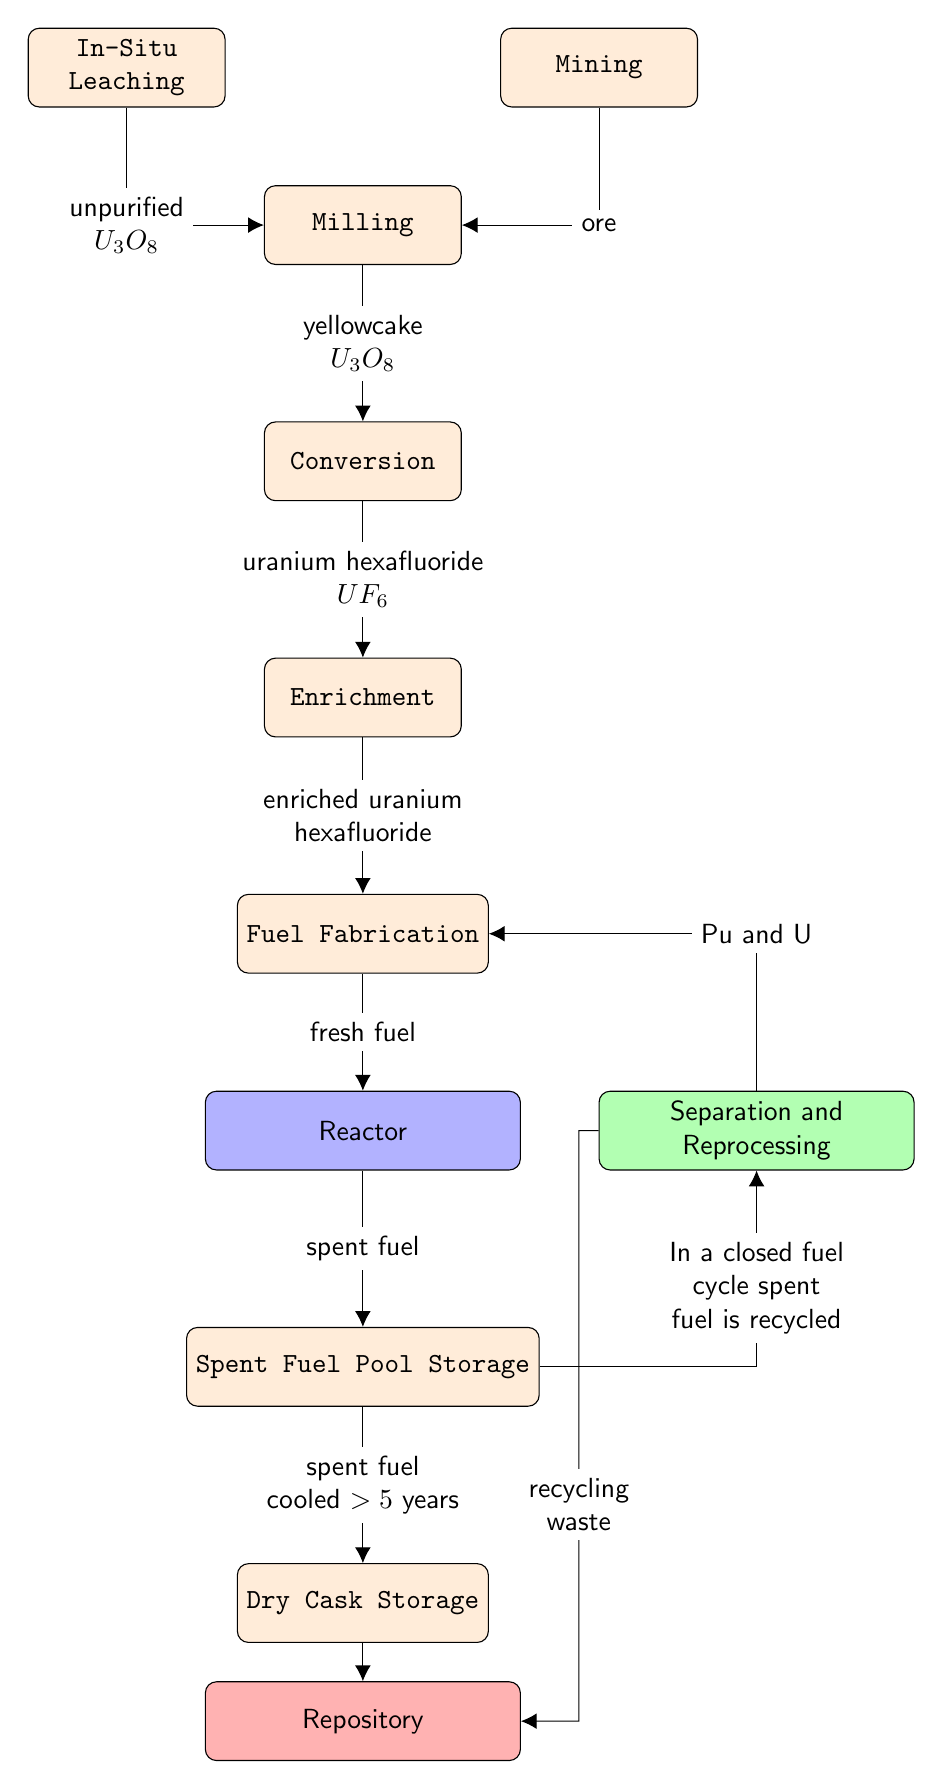
\begin{tikzpicture}[node distance=3cm,
    every node/.style={fill=white, font=\sffamily}, align=center]
  % Specification of nodes (position, etc.)
  \node (top) {};
  \node (leach)             [process, left of=top] {In-Situ\\Leaching};
  \node (mine)             [process, right of=top] {Mining};
  \node (mill)     [process, below of=top, yshift=1cm]          {Milling};
  \node (conv)      [process, below of=mill]   {Conversion};
  \node (enr)     [process, below of=conv]   {Enrichment};
  \node (fuelfab)          [process, below of=enr] {Fuel Fabrication};
  \node (reactor)      [bluebox, below of=fuelfab, yshift=0.5cm] {Reactor};
  \node (pool)       [process, below of=reactor] {Spent Fuel Pool Storage};
  \node (cask)    [process, below of=pool] {Dry Cask Storage};
  \node (reprocess)    [greenbox, right of=reactor, xshift=2cm] {Separation and\\Reprocessing};
  \node (repository) [redbox, below of=cask, yshift=1.5cm] {Repository};     
  % Specification of lines between nodes specified above
  % with aditional nodes for description 
\draw[->]     (leach) |- (mill) node[midway] {unpurified\\$U_3O_8$};
\draw[->]     (mine) |- (mill) node[midway] {ore};
\draw[->]     (mill) -- (conv) node[midway] {yellowcake\\$U_3O_8$};
\draw[->]      (conv) -- (enr) node[midway] {uranium hexafluoride\\$UF_6$};
\draw[->]     (enr) -- (fuelfab) node[midway] {enriched uranium\\hexafluoride};
  \draw[->]      (fuelfab) -- node[midway] {fresh fuel} (reactor);
  \draw[->]      (reactor) -- node[midway] {spent fuel} (pool);%\\uranium and\\fission products} (pool);
   \draw[->]       (pool) -- node[midway] {spent fuel\\cooled $>5$ years} (cask);
  \draw[->]       (pool) -| node[yshift=1cm, text width=3cm] {In a closed 
                            fuel cycle spent fuel is recycled} (reprocess);
  \draw[->]    (cask) -- (repository);
  \draw [->] (reprocess.west) -- ++(-0.25,0) -- node[yshift=-1cm] 
  {recycling\\waste} ++ (0,-7.5) -- (repository.0);
  \draw [->] (reprocess.north) |- node[midway] {Pu and U}  (fuelfab.east);

  %\draw[->] (reactor.east) -- ++(2.6,0) -- ++(0,2) -- ++(0,2) --                
  %   node[xshift=1.2cm,yshift=-1.5cm, text width=2.5cm]
  %   {The activity comes to the foreground}(fuelfab.east);
  \end{tikzpicture}
\end{document}

